% This file was created with tikzplotlib v0.10.1.
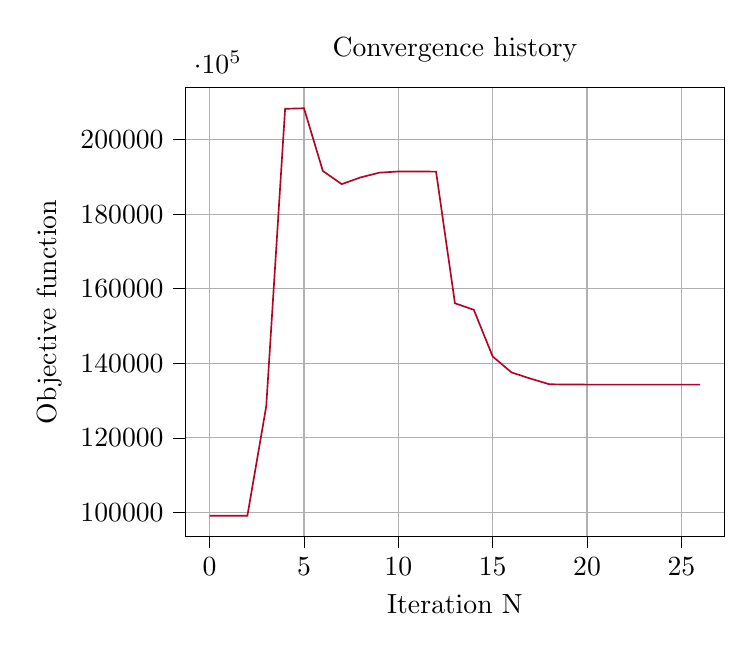
\begin{tikzpicture}

\definecolor{darkgray176}{RGB}{176,176,176}
\definecolor{firebrick180438}{RGB}{180,4,38}

\begin{axis}[
tick align=outside,
tick pos=left,
title={Convergence history},
x grid style={darkgray176},
xlabel={Iteration N},
xmajorgrids,
xmin=-1.3, xmax=27.3,
xtick style={color=black},
xtick={-5,0,5,10,15,20,25,30},
xticklabels={
  \(\displaystyle {\ensuremath{-}5}\),
  \(\displaystyle {0}\),
  \(\displaystyle {5}\),
  \(\displaystyle {10}\),
  \(\displaystyle {15}\),
  \(\displaystyle {20}\),
  \(\displaystyle {25}\),
  \(\displaystyle {30}\)
},
y grid style={darkgray176},
ylabel={Objective function},
ymajorgrids,
ymin=93598.0891447229, ymax=213893.295747853,
ytick style={color=black},
ytick={80000,100000,120000,140000,160000,180000,200000,220000},
yticklabels={
  \(\displaystyle {80000}\),
  \(\displaystyle {100000}\),
  \(\displaystyle {120000}\),
  \(\displaystyle {140000}\),
  \(\displaystyle {160000}\),
  \(\displaystyle {180000}\),
  \(\displaystyle {200000}\),
  \(\displaystyle {220000}\)
}
]
\addplot [semithick, firebrick180438]
table {%
0 99066.0530812288
1 99066.0530812288
2 99066.9997108456
3 128478.321460637
4 208275.793289342
5 208425.331811347
6 191602.588038656
7 188061.207461841
8 189870.311687249
9 191145.726818468
10 191456.155688858
11 191456.155688858
12 191421.42813153
13 156100.274503387
14 154345.444222848
15 141827.503562212
16 137535.788665613
17 135889.774612072
18 134369.911059166
19 134282.170033634
20 134279.363650898
21 134279.335957828
22 134279.325339022
23 134279.324439561
24 134279.324422043
25 134279.324421918
26 134279.324421918
};
\end{axis}

\end{tikzpicture}
